\documentclass[sigconf]{acmart}

\usepackage{hyperref}

\usepackage{endfloat}
\renewcommand{\efloatseparator}{\mbox{}} % no new page between figures

\usepackage{booktabs} % For formal tables

\settopmatter{printacmref=false} % Removes citation information below abstract
\renewcommand\footnotetextcopyrightpermission[1]{} % removes footnote with conference information in first column
\pagestyle{plain} % removes running headers

\begin{document}
\title{Big Data Analytics in Mobile device Application Development}


\author{ZhiCheng Zhu}
\affiliation{%
  \institution{Indiana University Bloomington}
  \streetaddress{936 S Clarizz Blvd}
  \city{Bloomington} 
  \state{Indiana} 
  \postcode{47401}
}
\email{zhuzhic@iu.edu}


\begin{abstract}

    With the development of the Internet, information increasingly becomes an important factor in determining the success of a product. A few years ago, manufacturing and the Internet have still belonged to two different separated industries, But as the mainstream consumer groups changed from old generation to Millennial generation, and the use of computers and the establishment and application of the Internet have produced a violent shock to the traditional way of product development, thus resulting in a new product development strategy. I have to say that the relation between the manufacturing and the Internet are getting closer and closer. One of the major changes might cause by using big data as a technique to develop right product and make effective promotion strategy.
    
\end{abstract}

\keywords{i523, hid229, Big data, Application Development, Technology}

\maketitle

\section{INTRODUCTION}
As a successful product designer,  you should not only consider the profits and losses of the current business but also have the foresight to predict the possible profit points. In order to maintain company's competitiveness for a long time, the enterprise must continue to grow and develop. According to past experience, the enterprise should get more profits to keep the growth. For some big company, it's easy to analyze what's working and what's not working, because they have a lot of past experience and data to analysis when they make the decision. With these data, they can create new promotions. 
In the past, if people want to predict whether a program was feasible or not, they had to go through the above process. Gain experience through a variety of failed or successful projects. It is safe to say that this approach has greatly increased the difficulty of developing new products and has also made start-up business only be a choice for the few people with the good financial or social status. Because not everyone has enough data to discover new consumer needs and has enough money to pay the huge cost to get the information. On the other hand, Generation changing in consumer groups have also brought some tremendous impact on product development. The difference between Millennial generation and Baby Boomers is enormous. And big data can play a big role in this area. Big data can dramatically reduce the cost which people used to spend on collecting data and use an intuitive way to told the product developers what changes have been happened to their consumers. These advantages are even more apparent in the area of software development.

\section{Big Data's advantages in reducing the cost}
With the development of the Internet, people are making data every moment. increasing quite quickly at a phenomenal rate. people always say we are in the era of big data but actually the real difference between now and before is just the change in the source of data, before the advent of the Internet, most of the past data was generated inside the enterprise and most of them were structured data, so In the past, large enterprises generally used the RDBMS (Relational Database Management System) to manage the data, this system is suitable for dealing with some data which is growing in an extremely slow way. so these companies do not have motivation or demand to process the data. with the emergence and rapid development of the Internet, especially the development of the mobile Internet, coupled with the large-scale use of various digital devices, the type of data is no longer just a simple structured data, these companies have to face more complex data types and faster changed customer psychology. Outdated decisions and information are bound to create disadvantages when competing with other companies, but the traditional data processing system is obviously not suitable for the era of big data. Corporate decision-makers must adopt new technologies to face the changes of the times and customer. For example, Hadoop technology is a new and widely accepted technology.
\begin{itemize}

  \item ``Hadoop is an open-source software framework for storing data and running applications on clusters of commodity hardware. It provides massive storage for any kind of data, enormous processing power and the ability to handle virtually limitless concurrent tasks or jobs.''
\end{itemize}
Adoption of new technologies brings not only higher efficiency but also lower costs.
\subsection{CHANGING IN TIME COST}
There are a lot of data, but usually, most of them are useless, only a small part of the data has the value. Collecting more data, the phenomenon will be more obvious, that is to say, irrelevant data growth rate is much higher than the growth of related data Speed. This also is a common phenomenon when we have large amounts of data. And the big data technique is used to deal with this new situation.
how to clean the data and find useful data more quickly in product development is even more important.Quickly identify the characteristics of the target customers and their possible needs for a variety of products. base on the analysis, we can develop some products that more suitable for marketplace needs, or we can be more accurate when we try to find our potential target customer. According to different consumer behavior, we can design different software, for example, during the financial turmoil we found that lots of users are price sensitive, we can design a kind of software that can provide local discount merchandise information in real time.If the target customer is a group which wants higher quality of life, we can push more high value-added product.
\section{Big Data in Application operation}
As we said before, the Millennial generation are very different from the baby boomers generation in terms of lifestyle and values. as a consequence, product designers should have different tactics for our product when we meet so many differences. The Millennial generation like to use the electronic mobile devices more frequently, and they are more willing to share their daily life on the Internet. These acts will undoubtedly produce a lot of information, produce useful data and timely data analysis will become extremely important in the future market.
\begin{figure}[!ht]
  \centering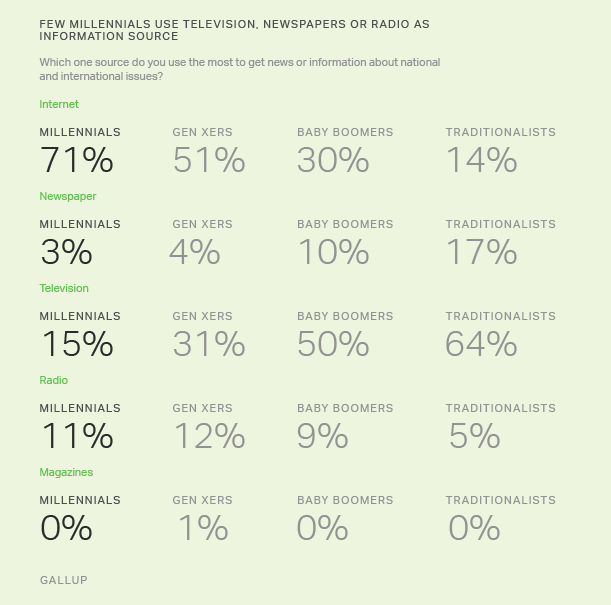
\includegraphics[width=\columnwidth]{images/relation.png}
  \caption{Difference between various generations \cite{part-reg}}
  \label{Figure 1}
\end{figure}
\subsection{Channel Promotion}
Which channels are best for promoting our application or what kind of application our target customer use before? This is extremely important for a newly launched application. The best way for us is to combine the different analytical methods with big data and help us find the most suitable channels. For example, SEM analysis, SEM analysis is a research and analysis methods which focus on customer satisfaction. This is a good way to make a classification for our users. One of the most typical examples is some recommender systems such as Pandora use songs or artist properties to create a radio station, all of these songs and artist have similar attributes. User feedback is used to adjust the content of the radio and recommend some music which is more attractive for the listener.
the recommendation system will reduce the possibility of recommending similar types of music when the user clicks on the "dislike" button to indicate that they are not interested in the song; the recommendation system will increase the possibility of recommending similar types of music when the user clicks on the "like" button to indicate that they are interested in the song, this is a form of content-based recommendation. Base on different attribute we can divide customers into distinct groups and then design different functions based on the different attribute.  this is somewhat similar to build a highly differentiated market and then makes our future marketing strategies more efficient.

\subsection{User Experience}
How to improve the user experience has become the key to determining whether a application will be success, because the good user experience can help us retain users and expand the user base, a good user experience may prompt the users to recommend your products to their friends. Users will generate a lot of data when they use the application, and these data will become the key to help us improve the user experience. For example, e-commerce platform user's data is always very valuable, the different brand television which user clicked before, the length of time they spent on different pages. all of these can help us understand the user, some data might relate to their interest and some might have a correlation with their family. all these attributes can help us to recommend a more suitable product next time. When a user starts to pay attention to some milk powder or other infant products, we can predict that this user's family may have a newborn baby recently. After that, we can provide personalized better service in the future. Especially for some new parents, most of them do not have experience so they might need suggestion.

\section{Conclusion}
Big data and machine learning are the two most popular fields in the Information Technology area. From the middle evil times' blocking of information to the explosion of data now, the amount of data in various fields and the scale of data sets have been increased at a phenomenal rate. The huge volume of data has brought huge potential opportunities and changes. With the proper use of the machine learning in big data can produce a lot of advantage. such as improve the efficiency. we can use the advantage of these data to help us make a better decision in different fields. one of a good example in scientific research is the data-driven research. In the scientific research, we can use the big data of the search engine to predict the ability widely used in the fields of medicine, astronomy and so on


\begin{acks}

  The authors would like to thank Dr. Gregor von Laszewski for his support and suggestions to write this paper as well as TAs' helpful suggestions on this paper.. 

\end{acks}

\bibliographystyle{ACM-Reference-Format}
\bibliography{report} 

\end{document}
